\chapter{پیش‌بینی عملکرد پروتئین‌ها با استفاده از گرافلت کرنل گاوسی}
پروتئین‌ها بخش مهمی از فعالیت‌های زیستی را تشکیل می‌دهند. درک نحوه کار آن‌ها وابسته به یافتن عملکرد و وظیفه هر کدام در سامانه‌های زیستی است. روش‌های آزمایشگاهی برای تشخیص عملکرد پروتئین پر هزینه هستند. بنابراین سعی می‌شود ابتدا با روش‌های محاسباتی، برای هر پروتئین عملکردی پیش‌بینی گردد و سپس در آزمایشگاه درستی این پیش‌بینی آزمون شود. این روش‌های محاسباتی پیش‌بینی، بر اساس تخصیص عملکرد به پروتئین ناشناخته بر مبنای عملکردهای شناخته شده برای پروتئین‌های مشابه، کار می‌کنند. معیارهای مختلفی برای اندازه‌گیری شباهت بین دو پروتئین تعریف شده‌است که از مهمترین آن‌ها می‌توان به روش‌های هم‌ترازی توالی\پانوشت{\متن‌لاتین{sequence alignment}} (مثل \متن‌لاتین{PSI-BLAST}\جستار{Altschul_1997} و \متن‌لاتین{FASTA}\جستار{Pearson_1988}) و هم‌ترازی ساختار\پانوشت{\متن‌لاتین{structure alignment}} (مثل \متن‌لاتین{DALI}\جستار{Holm_1996} و \متن‌لاتین{CE}\جستار{Shindyalov_1998}) اشاره کرد. این روش‌ها بر این مبنا استوارند که پروتئین‌های مشابه از لحاظ ساختاری، به احتمال زیاد از یک جد مشترک\پانوشت{\متن‌لاتین{common ancestor}} تکامل یافته‌اند پس باید عملکرد مشابهی داشته باشند\جستار{Reeck_1987}. بر همین اساس باید گفت در سیر تکامل، ساختار سه‌بعدی پروتئین‌ها کمتر دستخوش تغییر می‌شود\جستار{Illergaard_2009}. پس استفاده از آن برای اندازه‌گیری شباهت، نتایج بهتری بدست خواهد داد. ولی همیشه اینگونه نیست: ممکن است پروتئین‌ها با ساختار مشابه، عملکردهای متفاوت و پروتئین‌های با عملکرد مشابه، ساختار متفاوتی داشته باشند\جستار{Whisstock_2003}. برای در نظر گرفتن این حالت، روش‌های جدید، علاوه بر ساختار، اطلاعات دیگری از پروتئین (نظیر مقر اتصال\پانوشت{\متن‌لاتین{binding site}}\جستار{Binkowski_2003}، تعاملات پروتئینی\جستار{Xenarios_2002} و موتیف‌های اسیدآمینه\پانوشت{amino-acid motifs}\جستار{Yao_2003}) را در تصمیم‌گیری دخیل می‌کنند که می‌توان آن‌ها را به طور کلی به دو دسته تقسیم کرد. روش‌هایی نظیر \متن‌لاتین{ProKnown}\جستار{Pal_2005} و \متن‌لاتین{ProFunc}\جستار{Laskowski_2005} هر منبع اطلاعات را به صورت جداگانه استفاده می‌کنند. به این صورت که در هر منبع، پروتئین‌های مشابه با پروتئین مورد سؤال را مشخص کرده و سپس این اطلاعات را برای رتبه‌بندی پروتئین‌ها بر اساس شباهت استفاده می‌کنند. در روش دوم برای استفاده از اطلاعات مختلف، یک مدل احتمالاتی توام\پانوشت{\متن‌لاتین{joint probabilistic model}} تشکیل می‌شود. دابسن\پانوشت{Dobson} و دویگ \پانوشت{Doig} پروتئین‌ها را به شکل بردارهایی از خصوصیات فیزیکی و شیمیایی نشان دادند و از SVM برای یادگیری روی این بردارها استفاده کردند\جستار{Dobson_2003}. در این حالت می‌توان از هر منبع اطلاعاتی و هر نوع داده‌ای برای گسترش بردار منتسب به هر پروتئین استفاده کرد.

تلاش‌های زیادی برای بهبود مدل دابسن و دویگ هم از نظر سرعت اجرا و هم از نظر دقت، صورت گرفت. در این بین، روش‌های مبتنی بر گراف کرنل مورد توجه این پایان‌نامه هستند. در ادامه، ابتدا نحوه مدل‌کردن پروتئین به صورت گراف را توضیح داده و سپس از گراف کرنل گاوسی به همراه SVM برای ساخت ماشین تشخیص عملکرد استفاده می‌کنیم. در پایان به مقایسه روش‌های مشابه می‌پردازیم.

\section{ساختار پروتئین}\label{sec:protein-structure}
پروتئین‌ها مواد آلی بزرگ و یکی از انواع درشت مولکول‌های زیستی هستند که از \خمیده{اسیدهای آمینه} ساخته شده‌اند. هر اسیدآمینه، از یک کربن نامتقارن به نام کربن آلفا تشکیل یافته است که با چهار گروه مختلف کربوکسیل (\متن‌لاتین{COOH})، اتم هیدروژن، گروه آمینه (\متن‌لاتین{NH2}) و یک زنجیره جانبی (R) ارتباط برقرار می‌کند (شکل \ارجا{fig:aminoacid}). تغییر در زنجیره جانبی، نوع متفاوتی از اسیدآمینه را بوجود می‌آورد که مبنای نامگذاری آن‌هاست. حدود پانصد اسیدآمینه تاکنون شناسایی شده‌است\جستار{Wagner_1983} که ۲۰ عدد از آن‌ها در ساختمان پروتئین‌ها مشارکت دارند. در بین این ۲۰ اسیدآمینه، به غیر از گلیسین\پانوشت{Glycine} که زنجیره جانبی آن یک اتم هیدروژن است، مابقی در زنجیره جانبی خود چند اتم کربن دارند که آن‌ها را به ترتیب فاصله از اتم کربن آلفا با حروف یونانی بتا، گاما و دلتا نامگذاری می‌کنند.

\begin{figure}[h]
\center{
\begin{tikzpicture}[scale=1.5,transform shape,node distance=0.8cm,minimum size=0.40cm,inner sep=0,font=\tiny,
h/.style={circle,draw,thick,align=center,minimum size=0.30cm},
c/.style={circle,draw,thick,align=center,minimum size=0.40cm},
o/.style={circle,draw,thick,align=center,minimum size=0.60cm},
n/.style={circle,draw,thick,align=center,minimum size=0.50cm},
R/.style={rectangle,draw,thick,align=center,minimum size=0.80cm}]
% 2-node
    \node[h] (1) {H};
    \node[h] (2) [below of=1] {H};
    \node[n] (3) [below right=0.14cm and 0.25cm of 1] {N};
    \node[c] (4) [right of=3] {C};
    \node[h] (5) [below=-0.9cm of 4] {H};
    \node[R] (10) [below=0.4cm of 4] {R};
    \node[c] (6) [right of=4] {C};
    \node[o] (7) [below right=-0.9cm and 0.25cm of 6] {O};
    \node[o] (8) [below right=0.2cm and 0.25cm of 6] {O};
    \node[h] (9) [below=-1.1cm of 7] {H};
    \path (1) edge (3);
    \path (2) edge (3);
    \path (3) edge (4);
    \path (4) edge (5);
    \path (4) edge (6);
    \path (4) edge (10);
    \path (7) edge (6);
    \path (8) edge (6);
    \path (7) edge (9);
\end{tikzpicture}
}
\caption{
ساختار اسید‌های آمینه. هر اسیدآمینه از یک کربن آلفا تشکیل شده که با یک گروه آمینه(\متن‌لاتین{NH2})، یک گروه کربوکسیل (\متن‌لاتین{COOH}) و یک زنجیره جانبی (\متن‌لاتین{R}) ارتباط دارد.
}
\label{fig:aminoacid}
\end{figure}

با پیوند اسیدهای آمینه به صورت زنجیره‌‌ای بلند در فرآیند تولید پروتئین توسط سلول، یک \خمیده{پلی‌پپتید} بوجود می‌آید که در اصطلاح، \خمیده{ساختار اول} پروتئین را تشکیل می‌دهد. یعنی در ساده‌ترین حالت، پروتئین یک رشته طولانی ۲۰ حرفی از اسیدهای آمینه است. با برقراری پیوندهای هیدروژنی بین گروه آمینی و گروه کربوکسیل اسیدهای آمینه، نظم‌های موضعی در پروتئین به وجود می‌آید که به آن‌ \خمیده{ساختار دوم} پروتئین گفته می‌شود. \خمیده{مارپیچ آلفا}\پانوشت{\متن‌لاتین{alpha helix}} و \خمیده{صفحه بتا}\پانوشت{\متن‌لاتین{beta sheet}} دو نوع اصلی ساختار دوم هستند. با ورود زنجیره به فضای سلول و طی فرآیند تاشدگی\پانوشت{folding}، پروتئین شکل سه بعدی تقریباً ثابتی به خود می‌گیرد که به آن \خمیده{ساختار سوم} پروتئین گفته می‌شود. بعضی پروتئین‌ها از بیش از یک زنجیره پلی‌پتیدی بوجود می‌آیند. به نحوه قرار گرفتن این زنجیره‌ها در فضای سه‌بعدی، \خمیده{ساختار چهارم} پروتئین می‌گویند. شکل \ارجا{fig:protein} این مفاهیم را در قالب تصویر نشان می‌دهد.

\begin{figure}[h!]
\center{
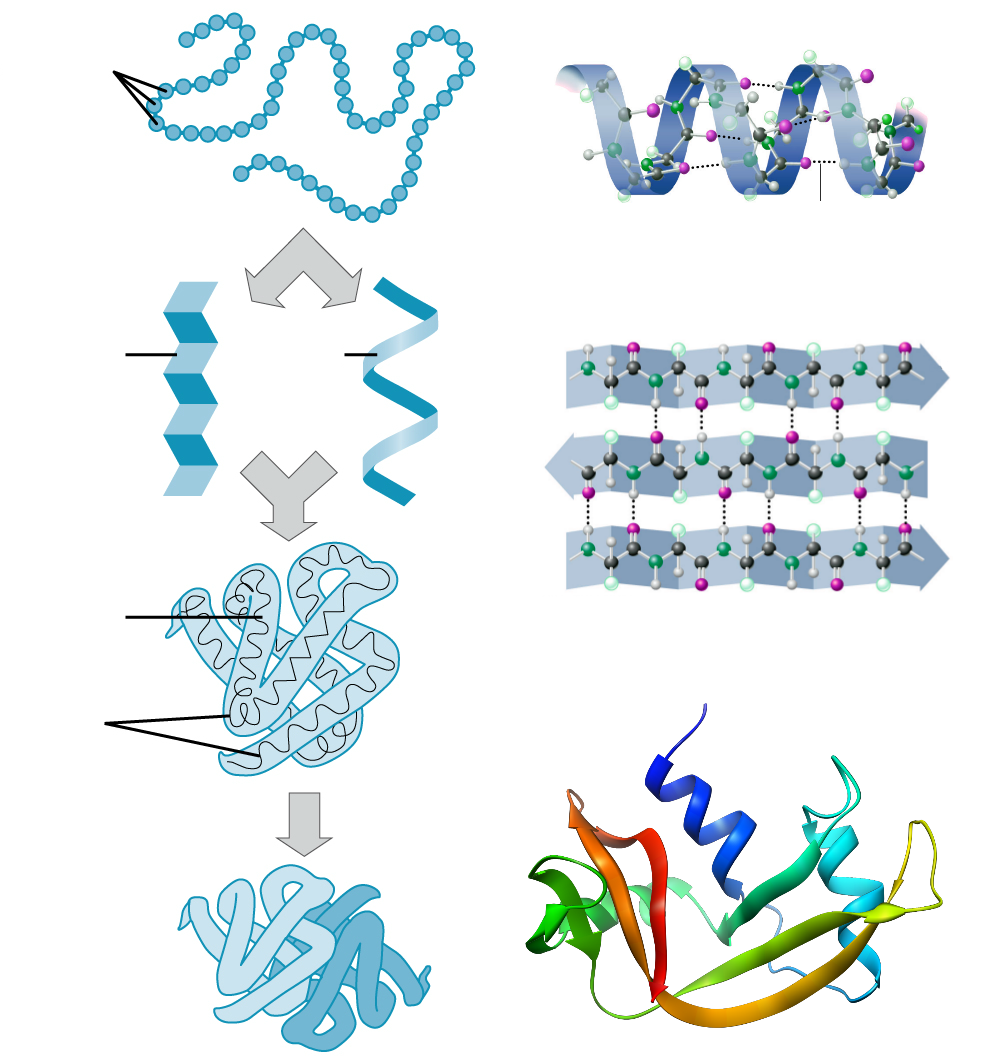
\includegraphics[scale=0.31]{./protein-structure-levels2.png}
}
\caption{
سطوح ساختاری پروتئین.
}
\label{fig:protein}
\end{figure}

\section{عملکرد پروتئین}
در فرآیندهای سلولی، پروتئین‌ها نقش اصلی را ایفا می‌کنند. در واقع تمام مولکول‌های دیگر موجود در سلول (به غیر از برخی RNA ها)، عناصری هستند که پروتئین‌ها برای انجام وظایف خود به ‌آن‌ها نیاز دارند و به وسیله‌ی آن‌ها فعالیت خود را انجام می‌دهند. مشخصه اصلی پروتئین‌ها که عملکرد‌های مختلف آن‌ها را نتیجه می‌دهد، توانایی اتصال به مولکول‌ها و پروتئین‌های دیگر است. قسمتی از پروتئین که این توانایی را فراهم می‌آورد، \خمیده{مقر اتصال} نامیده می‌شود که معمولاً به شکل یک حفره در سطح پروتئین واقع می‌گردد. نحوه فعالیت مقر اتصال و خصوصیات آن، توسط زنجیره جانبی اسید‌های آمینه اطراف آن مشخص می‌شود و به قدری خاص منظوره است که حتی یک تغییر کوچک در مولکول چسبنده، مانع از اتصال پروتئین خواهد شد. بنابراین ساختار سوم پروتئین مشخص کننده فعالیت‌ها و عملکرد‌های آن است.

می‌توان فعالیت پروتئین‌ها را به سه دسته کلی تقسیم کرد\جستار{Alberts_2014}:

\paragraph{سیگنال‌دهی و دریافت سیگنال}
به این وسیله پیغام‌هایی در سلول و حتی در سرتاسر بدن پخش می‌شود و واکنش سلول‌ها را به دنبال دارد. به عنوان مثال، انسولین پروتئینی است که نقش سیگنال‌دهی بین سلولی را بر عهده دارد. برخی دیگر از پروتئین‌ها بر روی غشاء سلولی ساکن هستند و نقش دریافت کننده سیگنال و در پی آن، فعال کردن واکنش‌های شیمیایی مناسب در داخل سلول را بر عهده دارند. بعضی پروتئین‌ها به عناصر دیگر می‌چسبند و آن‌ها را علامت‌گذاری می‌کنند. این عناصر علامت‌گذاری شده در فرآیند دیگری مورد استفاده قرار می‌گیرد. به عنوان مثال، پادتن‌ها پروتئین‌هایی هستند که با اتصال به عناصر خارجی، آن‌ها را برای از بین رفتن علامت‌گذاری می‌کنند.

\paragraph{نقش ساختاری}
ناخن، مو، پر و سایر ساختارهای سفت و محکم موجودات از پروتئین‌های ساختاری تشکیل شده‌است. اسکلت سلولی\پانوشت{\متن‌لاتین{cytoskeleton}} نیز از پروتئین‌های ساختاری آکتین\پانوشت{actin} و تبولین\پانوشت{tubulin} ساخته می‌شود.

\paragraph{نقش آنزیمی} 
آنزیم‌ها بزرگترین و مهم‌ترین دسته از پروتئین‌ها هستند. آن‌ها واکنش‌های شیمیایی را تسریع می‌کنند بدون آنکه خود در این واکنش‌ها تغییر یابند. آنزیم‌ها خاص منظوره هستند و معمولاً  هر کدام تنها روی یک یا چند واکنش تأثیرگذار است. حدود ۱۸۰۰۰ واکنش شناسایی شده‌اند که توسط آنزیم‌ها تسریع می‌شوند\جستار{Lang_2011} و برای ۸۷۰۰۰ آنزیم، ساختار سوم مشخص وجود دارد\جستار{Schomburg_2012}. آنزیم‌ها را می‌توان بر اساس عملکرد دسته‌بندی کرد. مهمترین دسته‌بندی آنزیم‌ها بر اساس عدد EC\پانوشت{\متن‌لاتین{Enzyme Commission number}} است. این عدد مشخص می‌کند که هر آنزیم روی چه واکنشی تأثیرگذار است.

\section{تبدیل پروتئین به گراف}
برای مدل کردن پروتئین به صورت گراف، معمولاً اسید‌های آمینه را به عنوان رئوس گراف در نظر می‌گیرند. بین هر دو رأس یال خواهد بود اگر اسیدهای آمینه متناظر حداکثر به فاصله تعریف شده $d$ از یکدیگر قرار گرفته باشند. به این فاصله، فاصله اتصال\پانوشت{\متن‌لاتین{contact distance}} می‌گوییم. برای اندازه‌گیری این فاصله، باید موقعیت هر اسیدآمینه در فضای سه بعدی را تعیین کرد. اما همانطور که در بخش \ارجا{sec:protein-structure} به آن اشاره شد، هر اسیدآمینه از چند اتم ساخته شده است. اینکه موقعیت اسیدآمینه توسط کدام اتم تعیین شود و فاصله اتصال چقدر باشد، موضوعی چالش برانگیز در تحقیقات بوده است. در بین مقالات مختلف، کربن آلفا 
($C_\alpha$)
، کربن بتا
($C_\beta$)
، ستون اسیدآمینه\پانوشت{backbone} ($BB$)، زنجیره جانبی ($SC$)، تمام اتم‌ها ($ALL$) و ترکیبات مختلف آن‌ها (مثل $C_\alpha+C_\beta$)، برای تعیین موقعیت اسید‌های آمینه استفاده شده‌اند. همچنین فواصل اتصال مختلفی بین ۴ تا ۱۶ آنگسترم در بین مقالات دیده می‌شود\جستار{Filippis_2012}.

\section{پیشبینی عملکرد پروتئین}
برای پیشبینی عملکرد 